\documentclass[border=5mm]{standalone}
\usepackage{tikz}
\begin{document}


\tikzset{every picture/.style={line width=0.75pt}} %set default line width to 0.75pt        

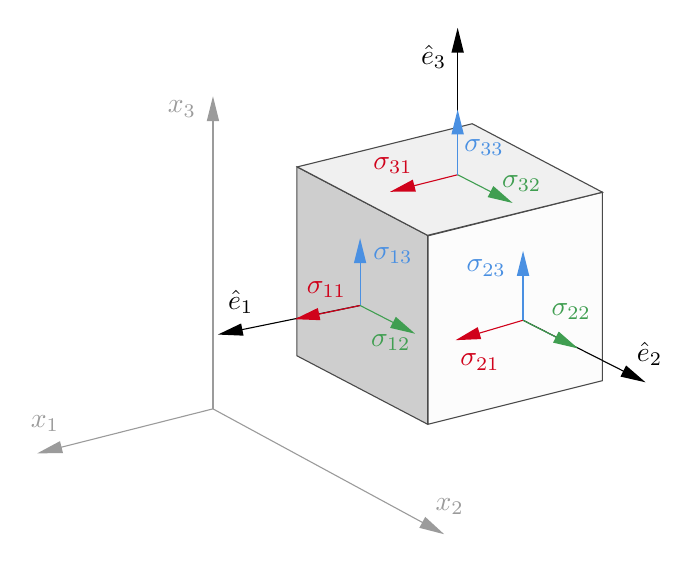
\begin{tikzpicture}[x=0.75pt,y=0.75pt,yscale=-1,xscale=1]
% ------------------------------------------------------------------------
% coordinate: axis-x3 (z)
\draw[color={rgb,255:red,155;green,155;blue,155},draw opacity=1](114,188)--(114,39.4);
\draw[shift={(114,37.4)},rotate = 90][fill={rgb,255:red,155;green,155;blue,155},fill opacity=1][line width=0.08][draw opacity=0](12,-3)--(0,0)--(12,3)--cycle;
% coordinate: axis-x2 (y)
\draw[color={rgb,255:red,155;green,155;blue,155},draw opacity=1](114,188)--(223.64,247.45);
\draw[shift={(225.4,248.4)},rotate = 208.47][fill={rgb,255:red,155;green,155;blue,155},fill opacity=1][line width=0.08][draw opacity=0](12,-3)--(0,0)--(12,3)--cycle;
% coordinate: axis-x1 (x)
\draw[color={rgb,255:red,155;green,155;blue,155},draw opacity=1](114,188)--(31.34,208.91);
\draw[shift={(29.4,209.4)},rotate = 345.8][fill={rgb,255:red,155;green,155;blue,155},fill opacity=1][line width=0.08][draw opacity=0](12,-3)--(0,0)--(12,3)--cycle;

% ------------------------------------------------------------------------
% cube: face-x1 (x)
\draw[color={rgb,255:red,74;green,74;blue,74},draw opacity=1][fill={rgb,255:red,158;green,158;blue,158},fill opacity=0.5](217.4,104.4)--(217.4,195.4)--(154.4,162.4)--(154.4,71.4)--cycle;
% cube: face-x2 (y)
\draw[color={rgb,255:red,74;green,74;blue,74},draw opacity=1][fill={rgb,255:red,250;green,250;blue,250},fill opacity=0.5](217.65,104.62)--(217.65,195.42)--(301.65,174.42)--(301.65,83.62)--cycle;
% cube: face-x3 (z)
\draw[color={rgb,255:red,74;green,74;blue,74},draw opacity=1][fill={rgb,255:red,240;green,240;blue,240},fill opacity=1](217.4,104.4)--(154.65,71.42)--(238.91,50.63)--(301.65,83.62)--cycle;

% ------------------------------------------------------------------------
% arrow: e_{1}
\draw[color={rgb,255:red,0;green,0;blue,0},draw opacity=1](184.9,138.2)--(118.36,151.8);
\draw[shift={(116.4,152.2)},rotate = 348.45][fill={rgb,255:red,0;green,0;blue,0},fill opacity=1][line width=0.08][draw opacity=0](12,-3)--(0,0)--(12,3)--cycle;
% arrow: e_{2}
\draw[color={rgb,255:red,0;green,0;blue,0},draw opacity=1](263.4,145.3)--(320.62,174.3);
\draw[shift={(322.4,175.2)},rotate = 206.87][fill={rgb,255:red,0;green,0;blue,0},fill opacity=1][line width=0.08][draw opacity=0](12,-3)--(0,0)--(12,3)--cycle;
% arrow: e_{3}
\draw[color={rgb,255:red,0;green,0;blue,0},draw opacity=1](231.9,75.2)--(231.9,6.4);
\draw[shift={(231.9,4.4)},rotate = 90][fill={rgb,255:red,0;green,0;blue,0},fill opacity=1][line width=0.08][draw opacity=0](12,-3)--(0,0)--(12,3)--cycle;

% ------------------------------------------------------------------------
% arrow: sigma_{11} 
\draw[color={rgb,255:red,208;green,2;blue,27},draw opacity=1](184.9,138.2)--(155.36,144.39);
\draw[shift={(153.4,144.8)},rotate = 348.17][fill={rgb,255:red,208;green,2;blue,27},fill opacity=1][line width=0.08][draw opacity=0](12,-3)--(0,0)--(12,3)--cycle;
% arrow: sigma_{12}
\draw[color={rgb,255:red,64;green,158;blue,81},draw opacity=1](184.9,138.2)--(209.62,150.89);
\draw[shift={(211.4,151.8)},rotate = 207.17][fill={rgb,255:red,64;green,158;blue,81},fill opacity=1][line width=0.08][draw opacity=0](12,-3)--(0,0)--(12,3)--cycle;
% arrow: sigma_{13}
\draw[color={rgb,255:red,74;green,144;blue,226},draw opacity=1](184.9,138.2)--(184.9,107.8);
\draw[shift={(184.9,105.8)},rotate = 90][fill={rgb,255:red,74;green,144;blue,226},fill opacity=1][line width=0.08][draw opacity=0](12,-3)--(0,0)--(12,3)--cycle;

% ------------------------------------------------------------------------
% arrow: sigma_{21}
\draw[color={rgb,255:red,208;green,2;blue,27},draw opacity=1](263.4,145.3)--(232.82,154.33);
\draw[shift={(230.9,154.9)},rotate = 343.54][fill={rgb,255:red,208;green,2;blue,27},fill opacity=1][line width=0.08][draw opacity=0](12,-3)--(0,0)--(12,3)--cycle;
% arrow: sigma_{22}
\draw[color={rgb,255:red,64;green,158;blue,81},draw opacity=1](263.4,145.3)--(288.12,157.99);
\draw[shift={(289.9,158.9)},rotate = 207.17][fill={rgb,255:red,64;green,158;blue,81},fill opacity=1][line width=0.08][draw opacity=0](12,-3)--(0,0)--(12,3)--cycle;
% arrow: sigma_{23}
\draw[color={rgb,255:red,74;green,144;blue,226},draw opacity=1](263.4,145.3)--(263.4,113.9);
\draw[shift={(263.4,111.9)},rotate = 90][fill={rgb,255:red,74;green,144;blue,226},fill opacity=1][line width=0.08][draw opacity=0](12,-3)--(0,0)--(12,3)--cycle;

% ------------------------------------------------------------------------
% arrow: sigma_{31}
\draw[color={rgb,255:red,208;green,2;blue,27},draw opacity=1](231.9,75.2)--(201.34,82.91);
\draw[shift={(199.4,83.4)},rotate = 345.84][fill={rgb,255:red,208;green,2;blue,27},fill opacity=1][line width=0.08][draw opacity=0](12,-3)--(0,0)--(12,3)--cycle;
% arrow: sigma_{32}
\draw[color={rgb,255:red,64;green,158;blue,81},draw opacity=1](231.9,75.2)--(256.62,87.89);
\draw[shift={(258.4,88.8)},rotate = 207.17][fill={rgb,255:red,64;green,158;blue,81},fill opacity=1][line width=0.08][draw opacity=0](12,-3)--(0,0)--(12,3)--cycle;
% arrow: sigma_{33}
\draw[color={rgb,255:red,74;green,144;blue,226},draw opacity=1](231.9,75.2)--(231.9,45.8);
\draw[shift={(231.9,43.8)},rotate = 90][fill={rgb,255:red,74;green,144;blue,226},fill opacity=1][line width=0.08][draw opacity=0](12,-3)--(0,0)--(12,3)--cycle;

% ------------------------------------------------------------------------
% label: arrow e_{1}
\draw(120,129.4) node [anchor=north west][inner sep=0.75pt][color={rgb,255:red,0;green,0;blue,0},opacity=1]{$\hat{e}_{1}$};
% label: arrow e_{1}
\draw(317,154.5) node [anchor=north west][inner sep=0.75pt][color={rgb,255:red,0;green,0;blue,0},opacity=1]{$\hat{e}_{2}$};
% label: arrow e_{1}
\draw(213,11.4) node [anchor=north west][inner sep=0.75pt][color={rgb,255:red,0;green,0;blue,0},opacity=1]{$\hat{e}_{3}$};

% ---------------
% label: arrow sigma_{11}
\draw(158,125.5) node [anchor=north west][inner sep=0.75pt][color={rgb,255:red,208;green,2;blue,27},opacity=1]{$\sigma_{11}$};
% label: arrow sigma_{12}
\draw(189,151) node [anchor=north west][inner sep=0.75pt][color={rgb,255:red,64;green,158;blue,81},opacity=1]{$\sigma_{12}$};
% label: arrow sigma_{13}
\draw(190,109) node [anchor=north west][inner sep=0.75pt][color={rgb,255:red,74;green,144;blue,226},opacity=1]{$\sigma_{13}$};

% ---------------
% label: arrow sigma_{21}
\draw(231.9,160.3) node [anchor=north west][inner sep=0.75pt][color={rgb,255:red,208;green,2;blue,27},opacity=1]{$\sigma_{21}$};
% label: arrow sigma_{22}
\draw(275.9,136) node [anchor=north west][inner sep=0.75pt][color={rgb,255:red,64;green,158;blue,81},opacity=1]{$\sigma_{22}$};
% label: arrow sigma_{23}
\draw(234.9,115) node [anchor=north west][inner sep=0.75pt][color={rgb,255:red,74;green,144;blue,226},opacity=1]{$\sigma_{23}$};

% ---------------
% label: arrow sigma_{31}
\draw(190,65.5) node [anchor=north west][inner sep=0.75pt][color={rgb,255:red,208;green,2;blue,27},opacity=1]{$\sigma_{31}$};
% label: arrow sigma_{32}
\draw(252,74.5) node [anchor=north west][inner sep=0.75pt][color={rgb,255:red,64;green,158;blue,81},opacity=1]{$\sigma_{32}$};
% label: arrow sigma_{33}
\draw(233.9,57) node [anchor=north west][inner sep=0.75pt][color={rgb,255:red,74;green,144;blue,226},opacity=1]{$\sigma_{33}$};

% ---------------
% label: coordinate x_{1}
\draw(25,190) node [anchor=north west][inner sep=0.75pt][color={rgb,255:red,155;green,155;blue,155},opacity=1]{$x_{1}$};
% label: coordinate x_{2}
\draw(220,230) node [anchor=north west][inner sep=0.75pt][color={rgb,255:red,155;green,155;blue,155},opacity=1]{$x_{2}$};
% label: coordinate x_{3}
\draw(91,38.4) node [anchor=north west][inner sep=0.75pt][color={rgb,255:red,155;green,155;blue,155},opacity=1]{$x_{3}$};
% ------------------------------------------------------------------------
\end{tikzpicture}
\end{document}